\chapter{Image classification}


\section{Supervised datasets}

\begin{description}
    \item[Dataset] \marginnote{Dataset}
        Given a set of labeled data, it can be split into:
        \begin{descriptionlist}
            \item[Train set] $D^\text{train} = \{ (\text{x}_\text{train}^{(i)}, y_\text{train}^{(i)}) \mid i = 1, \dots, N \}$.
            \item[Test set] $D^\text{test} = \{ (\text{x}_\text{test}^{(i)}, y_\text{test}^{(i)}) \mid i = 1, \dots, M \}$.
        \end{descriptionlist}

        It is assumed that the two sets contain i.i.d. samples drawn from the same unknown distribution.
\end{description}


\subsection{Modified NIST (MNIST)}

\begin{minipage}{0.45\linewidth}
    \centering
    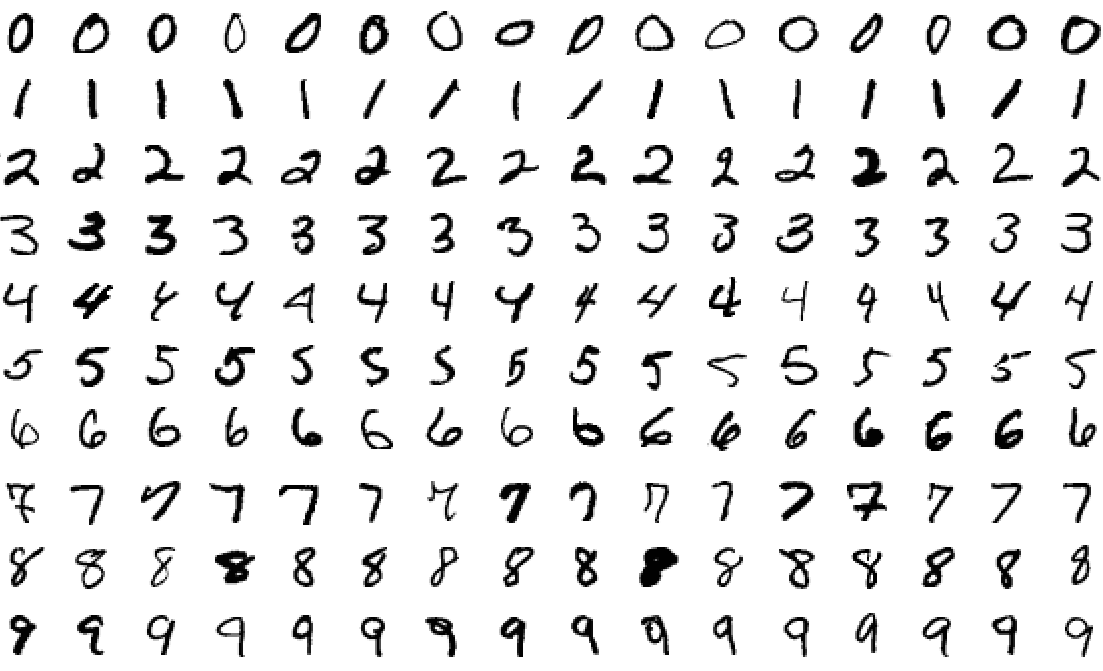
\includegraphics[width=0.9\linewidth]{./img/mnist.png}
\end{minipage}
\begin{minipage}{0.5\linewidth}
    \begin{descriptionlist}
        \item[Content] Handwritten digits from 0 to 9.
        \item[Number of classes] 10.
        \item[Train set size] 50k.
        \item[Test set size] 10k.
        \item[Image format] $28 \times 28$ grayscale.
    \end{descriptionlist}
\end{minipage}


\subsection{CIFAR10}

\begin{minipage}{0.45\linewidth}
    \centering
    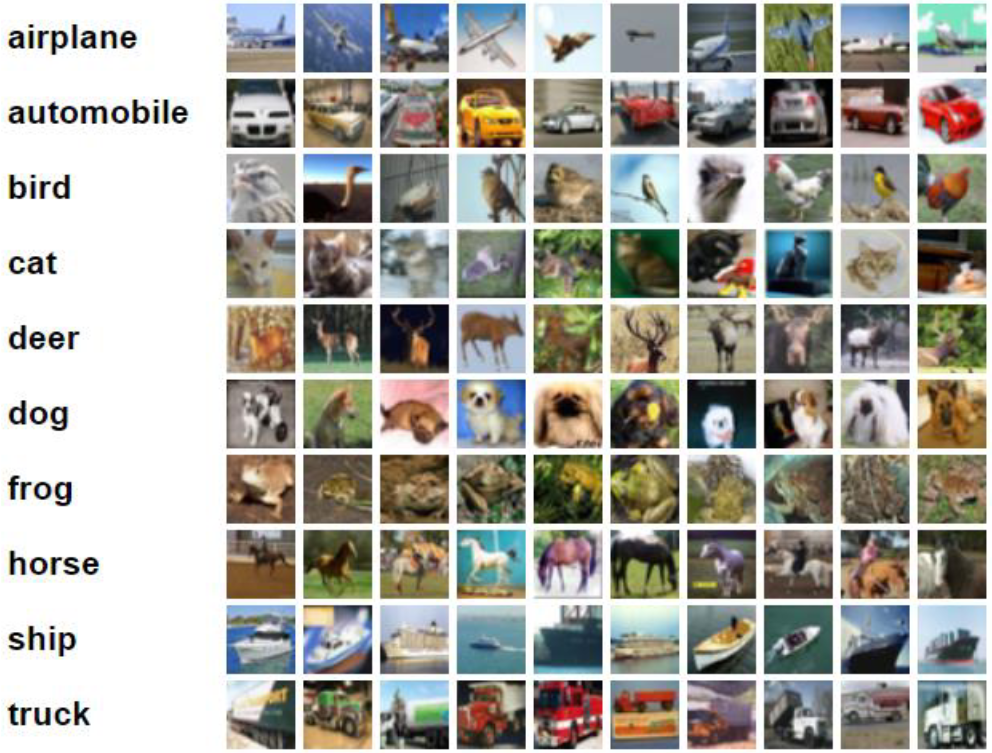
\includegraphics[width=0.9\linewidth]{./img/cifar10.png}
\end{minipage}
\begin{minipage}{0.5\linewidth}
    \begin{descriptionlist}
        \item[Content] Objects of various categories.
        \item[Number of classes] 10.
        \item[Train set size] 50k.
        \item[Test set size] 10k.
        \item[Image size] $32 \times 32$ RGB.
    \end{descriptionlist}
\end{minipage}


\subsection{CIFAR100}

\begin{minipage}{0.45\linewidth}
    \centering
    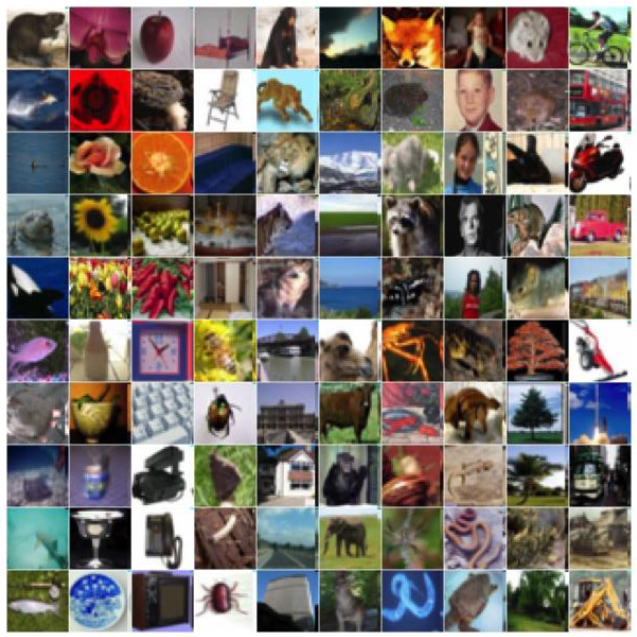
\includegraphics[width=0.7\linewidth]{./img/cifar100.png}
\end{minipage}
\begin{minipage}{0.5\linewidth}
    \begin{descriptionlist}
        \item[Content] Objects of various categories.
        \item[Number of classes] 100 (20 super-classed with 5 sub-classes).
        \item[Train set size] 50k.
        \item[Test set size] 10k.
        \item[Image size] $32 \times 32$ RGB.
    \end{descriptionlist}
\end{minipage}


\subsection{ImageNet 21k}

\begin{descriptionlist}
    \item[Content] Objects of various categories.
    \item[Number of classes] 21k synsets from WordNet organized hierarchically.
    \item[Dataset size] 14 millions.
    \item[Image size] Variable resolution RGB. Average size of $400 \times 350$.
\end{descriptionlist}

\begin{figure}[H]
    \centering
    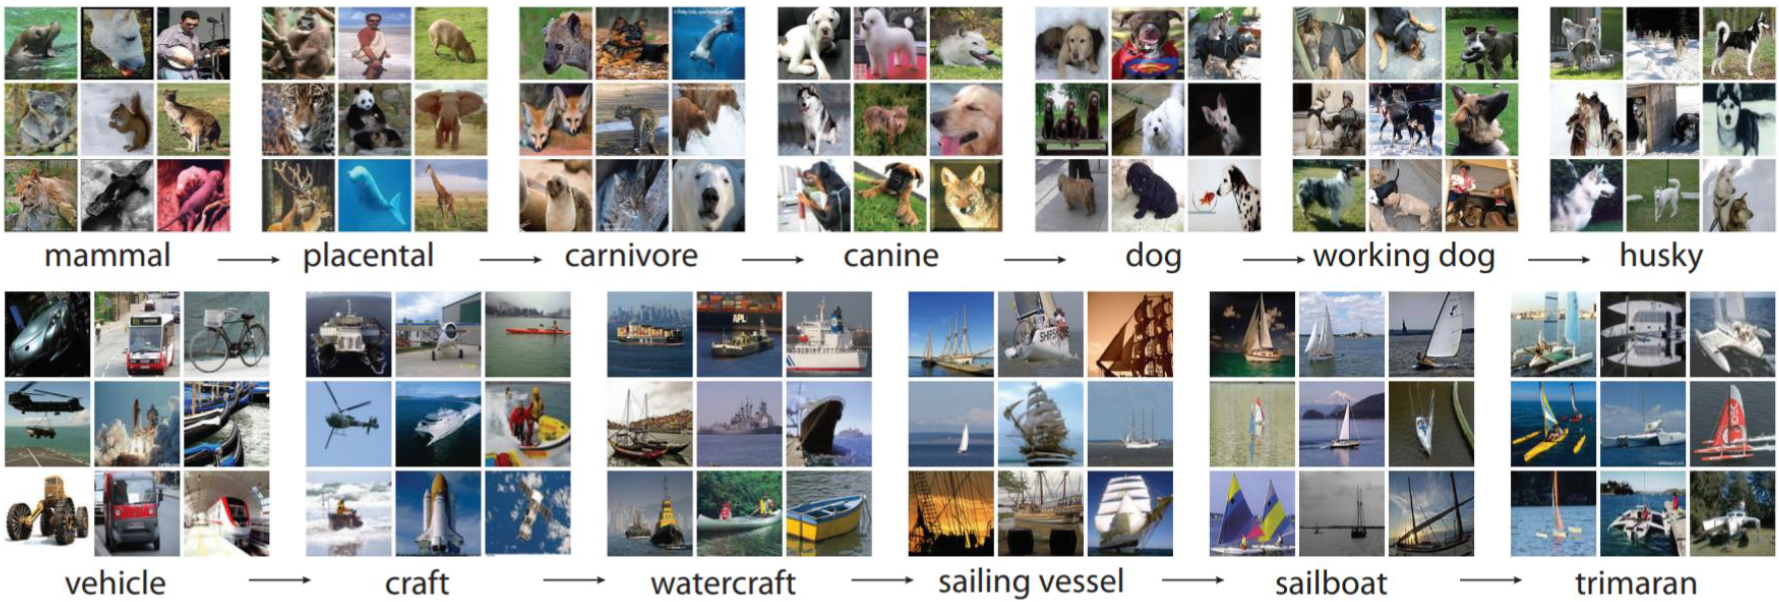
\includegraphics[width=0.85\linewidth]{./img/imagenet21k.png}
\end{figure}


\subsection{ImageNet 1k}

\begin{minipage}{0.45\linewidth}
    \centering
    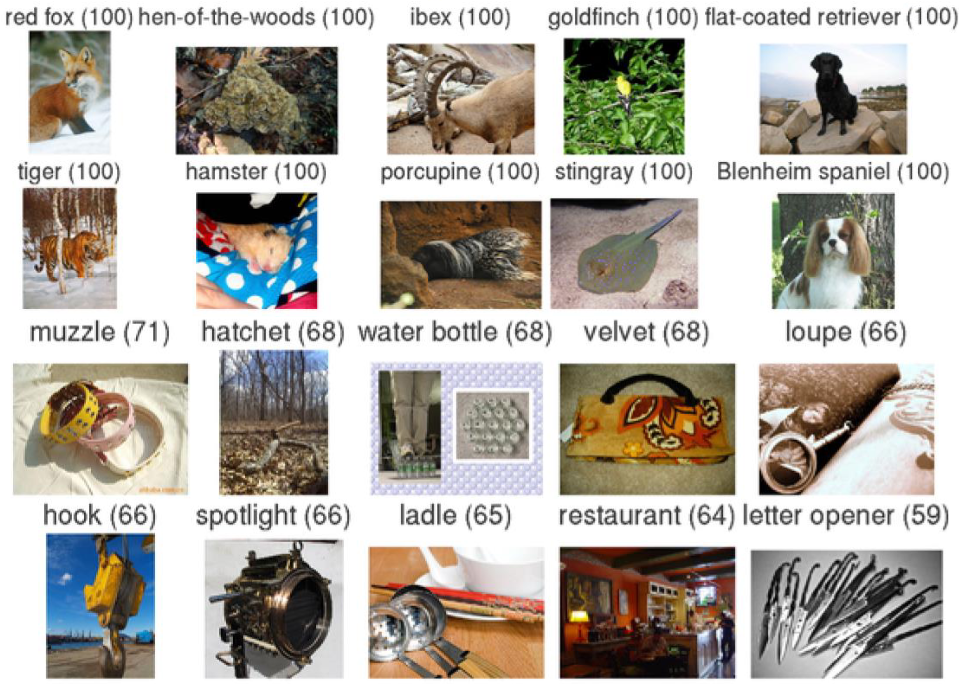
\includegraphics[width=\linewidth]{./img/imagenet1k.png}
\end{minipage}
\begin{minipage}{0.5\linewidth}
    \begin{descriptionlist}
        \item[Content] Objects of various categories.
        \item[Number of classes] 1000.
        \item[Train set size] $1.3$ millions.
        \item[Validation set size] 50k.
        \item[Test set size] 100k.
        \item[Image size] Variable resolution RGB. Often resized to $256 \times 256$.
    \end{descriptionlist}
\end{minipage}

\begin{remark}
    Performance is usually measured as top-5 accuracy as making a single prediction might be ambiguous due to the fact that the images can contain multiple objects.
\end{remark}


